% Drawing 144/03-2 -- folder 144, batch 03, archive page 46 (PDF page 47).
% Transcription: Le demi-plan supérieur : axe réel, axe imaginaire, demi-cercle unité ; la bande verticale hachurée au-dessus de l'arc qui va de $i$ au point marqué $j$ (domaine fondamental).
% Kind: upper half-plane, fundamental strip. Method 2 (schematic redraw from the facsimile). Status: ok.
% Notes: Real axis, imaginary axis (pencil), unit half-circle; the vertical strip above the arc from i to the marked point j is hatched (its left side on the imaginary axis).
% Coordinates: 1 unit = 1 mm = 1/100 of the crop width (bbox in page fractions: [0.18, 0.05, 0.48, 0.3]).
% Redrawn by Claude (claude-opus-5-5), issue #73, 2026-11-07; not checked by a human; not compiled (no TeX in the session).
% Rights: reproduces part of the work -- behind RENDER_TRANSCRIPTS, never published by itself.
\documentclass[tikz,border=3pt]{standalone}
\usepackage{amsmath,amssymb}
\usetikzlibrary{patterns,arrows.meta}
\tikzset{pencil/.style={black!45}, struck/.style={black!35}, mark/.style={circle,draw,inner sep=1.3pt}, pt/.style={circle,fill,inner sep=0.9pt}, opt/.style={circle,draw,fill=white,inner sep=1.1pt}}
\begin{document}
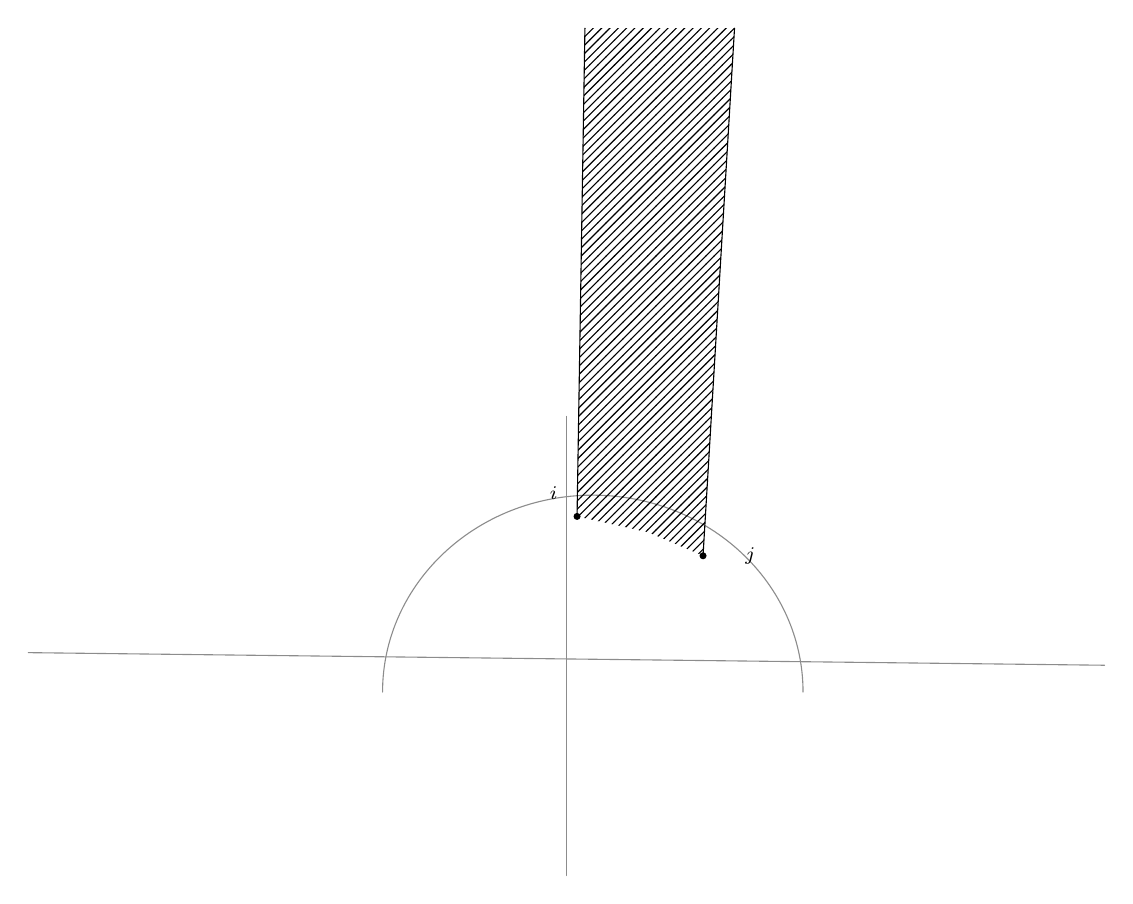
\begin{tikzpicture}[x=1mm,y=1mm,line cap=round,line join=round,font=\scriptsize]
\draw[pencil] (-26.7,-91.3) -- (110,-92.9);
\draw[pencil] (41.7,-61.3) -- (41.7,-119.6);
\draw[pencil] (71.7,-96.3) arc[start angle=0, end angle=180, x radius=26.7, y radius=25];
\draw (44,-12) -- (43,-74);
\draw (63,-12) -- (59,-79);
\fill[pattern=north east lines] (44,-12) -- (63,-12) -- (59,-79) -- (52,-76) -- (43,-74) -- cycle;
\node[pt] at (43,-74) {};
\node[pt] at (59,-79) {};
\node[inner sep=1pt] at (40,-71) {\scriptsize $i$};
\node[inner sep=1pt] at (65,-79) {\scriptsize $j$};
\end{tikzpicture}
\end{document}
